\documentclass [12pt] {article}
\usepackage{amsmath,graphicx,natbib} 

\title{GEO242 Lupita Final Project: 

The 1994 Northridge Earthquake and Omori Law}
\author{Lupita Bravo}
\date{December 2025}


\begin{document}

\maketitle

\section*{Background}
The 1994 $M_w$ 6.7 Northridge earthquake occurred in an urban area near Los Angeles.\citep{Hauksson_1995,Hartzell_1996} This is one of the major events that had occurred in the San Fernando Valley area with the major event preceding it being the $M_w$ 6.6 1971 San Fernando Earthquake.\citep{Hauksson_1995,Thio_1996,Hough_2024} This event, similar to the 1971 San Fernando earthquake has major impacts as it also had major losses. To this day, people still remember the 1994 earthquake and there have been serval outreach materials and events made to remember the 1994 event. \citep{Hough_2024}
\begin{figure}
    \centering
    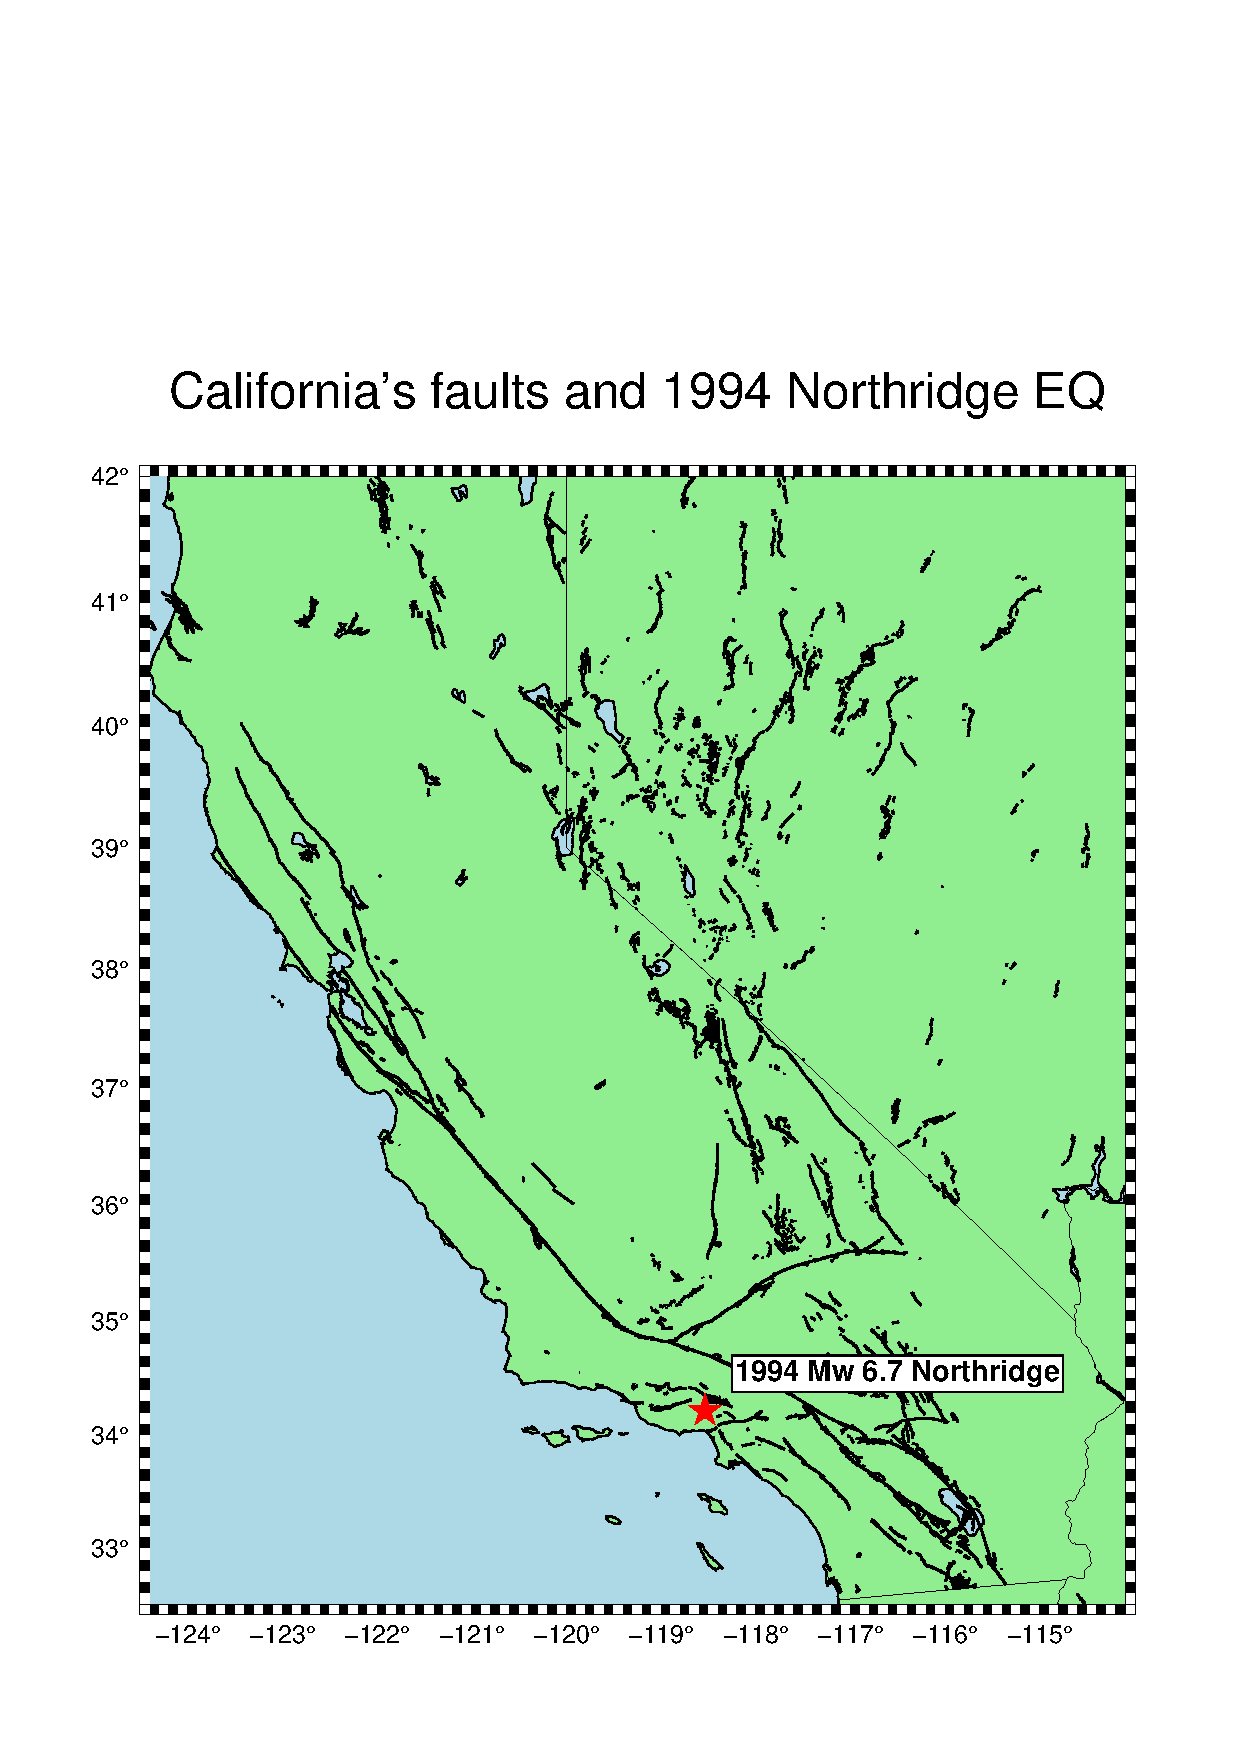
\includegraphics[width=0.75\linewidth]{Figures/Basic_map.ps.png}
    \caption{This is a map of California where the black lines are faults and the red star is the location of the 1994 Northridge Earthquake.}
    \label{fig:basicmap}
\end{figure}

For my final project, I am going to look at the aftershocks for the 1994 Northridge Earthquake and fit a trend to the aftershocks. I hypothesize that the magnitude and frequency of the event will follow Omori law. Omori law, as stated in \cite{Scholz_2019} has to do with the decay of aftershocks for a given main shock. The equation given in \cite{Scholz_2019} is shown in equation \ref{eq:Omori}. Here \(n(t)\) is the number of earthquake sin a given time, t is the time since the main shock, \(c\) is a small positive number and \(K,\) and \(p\) are all constants. \citep{Scholz_2019} Typically the decay is a curved line. There have been several versions of the Omori Law equation, for example in \cite{Shcherbakov_2004}, they mention a modified form that also includes magnitude. Overall, typically we observe a curved decay over time where there are more aftershocks, usually at somewhat larger magnitudes but less than the main shock, right after an earthquake compared to after much time has passed where we see less number of after shocks and they are smaller. 
\begin{equation}
    n(t) = \frac{K}{(c+t)^p}
     \label{eq:Omori}
\end{equation}
\section*{Goals}
My goals for this project include:
    \begin{itemize}
        \item Generate maps using GMT for the 1994 Northridge Earthquake
        \item Use data manipulation commands, like {\it ``awk" }, to organize the data downloaded from the Southern California Data Center (SCEDC) 
        \item Visualize the groupings for the events in three month increments on both a map and on a plot against time 
        \item Fit a line through the data to show the decaying trend as discussed in Omori Law
        \item Fit a plane to the data
    \end{itemize}
\section*{Methods}
\subsection*{Data}
I downloaded data for the area where the 1994 Northridge earthquake occurred from the Southern California Data Center (SCEDC). Prior to downloading data from this website, I had downloaded an earthquake catalog from USGS, however the SCEDC catalog had more events so I ended up deciding to work with the SCEDC catalog instead. Table \ref{table:SCEDC} shows the values inputted into the SCEDC website when downloading data. While there were other parameters I could use for filtering out data, the parameters I focused on were the start date, end date, and the latitude and longitude for my area of interest. 
\begin{table}[h]
	\caption{This table shows the parameters used when downloading the data from SCEDC.}
    \label{table:SCEDC}
	\begin{center}
		\begin{tabular}{|c|c|c|c|c|c|}
			\hline
			Start Date & End Date & North & South & East & West\\
			\hline
			1994-01-10-00-00-00 & 1995-01-18-00-00-00 & 34.5 & 34.1 & -118.2 & -118.8\\
			\hline
		\end{tabular}
	\end{center}
\end{table}

I wanted to visualize the data before working on organizing it and breaking it down into three different increments. Fig \ref{fig:AllEQs} plots all of the earthquakes within the time span and location I picked for this event\footnote{I just wanted to note that while I filtered it so the time window started form January 10, 1994, the earliest event I had in my catalog was on January 14, 1994} . 
\begin{figure}
    \centering
    \includegraphics[width=1\linewidth]{Figures/All_EQs_1_year_M_vs_T.pdf}
    \caption{This plot shows the raw data for the time span I selected when downloading the data. Here I'm plotting magnitude on the y axis and time on the x axis. Each black circle is an earthquake that occurred.}
    \label{fig:AllEQs}
\end{figure}
After visualizing the data, I returned to the\textit{``.sh"} file where I had been working on organizing the text file for the whole year and broke it into 4 smaller groups with respect to time. Table \ref{table:Dates} shows the date range for each text file. 
In addition to the earthquake catalog from SCEDC, I also downloaded data to make the maps. I obtained the focal mechanism for the event from the Global CMT Webpage. For the DEM of the area, I used ``sardem'' do download the DEM and used the to generate my color palette for elevation. The fault files used in the maps were the files we had previously downloaded during one of the lectures.
\begin{table}[hp]
	\caption{This table shows different groups for the earthquakes for Figures \ref{fig:SeisMap} and \ref{fig:EQsColor}}
     \label{table:Dates}
	\begin{center}
		\begin{tabular}{|c|c|c|}
			\hline
			Name & Start Date & End Date \\
			\hline
			Pre-1994 Northridge EQ & 1/10/1994 & 1/17/1994 \\ 
            \hline
			Jan 1994 - Apr 1994 & 1/17/1994 & 4/16/1994 \\ 
			\hline
            Apr 1994 - Jul 1994 & 4/17/1994 & 7/16/1994 \\ 
			\hline
            Jul 1994 - Oct 1994  & 7/17/1994 & 10/16/1994 \\ 
			\hline
            Oct 1994 - Jan 1995 & 10/17/1994 & 1/17/1995\\ 
			\hline
		\end{tabular}
	\end{center}
\end{table}

\subsection*{Work Flow}
Initially, my goal was to keep all the coding on one Jupyter Notebook. Using that approach, however resulted in a very messy and long notebook. I then decided to combine the use of both \textit{``.sh''} files and Jupyter Notebook as there were certain instances\footnote{This is a footnote, I primarily included it just to show that I was able to get it to work in LaTex. It was easier to do some of the data organizing in the \textit{``.sh''} file and to do my maps using a \textit{``.sh''} file. In some cases it was easier to use Jupyter Notebook since I was able to load in the text files as a data frame and do the analysis there similar to what we did in class.}, where one worked better than the other. 

After I had the different text files that broke down my main catalog into the smaller increments, I worked on getting the maps running. For the maps, I referenced a majority of what we did in class and for the assignments and made modifications to get it to work for the Northridge. 

After making the maps, I returned to Jupyter Notebook to work on first, plotting a plot similar to what the seismicity map (Fig \ref{fig:SeisMap}) is showing, however Fig \ref{fig:EQsColor} allows for an easier view of what occurs with the aftershocks over time. 

Next, I worked on the Omori Law fit. The goal here was to fit a line to the data to show how the number of earthquakes decays over time as shows in equation \ref{eq:Omori}. Due to Omroi's Law not being a linear, I looked through the documentation for one of the dependencies we used in class \textit{(scipy.optimize}) and referenced the \textit{curve fit} examples. First I defined a function for the Omori Law equation \ref{eq:Omori}. Next, I needed to get the time data in a format I could use. I took the difference between the different events in respect to the main shock and converted these differences into a format I can use, this would be our \(``t".\) Since Omori Law involved aftershocks, I removed the events that occurred before the main shock. I still need the\(n(t)\) which would be the number of earthquakes at a certain time. To calculate this, I used a for loop that could count the number of earthquakes each day after the earthquake occurred. This loop saved \(t\) and \(n(t)\). After obtaining these values, I calculated for the \(k\), \(c\), and \(p\). Lastly, using the values calculated and function created earlier, I fit a line through the data. 

Lastly, I worked on fitting a plane to the data. Since the data locations were in latitude and longitude, I converted them to a UTM coordinate system, my reasoning being that they way the values would be positive. Using an example on how to do this, I also attempted to convert the UTM coordinates back to latitude and longitude. After seeing that this worked for one set of coordinates, I did it for all events. Prior to that, I had to convert the data frame columns for the latitude and longitude into numpy arrays for it to work. After converting them, I added these values into my data frame as new columns so I'd have it all in one place. 
\begin{equation}
    z = ax + by + c
    \label{eq:Plane}
\end{equation}
After converting the latitude and longitudes, I set up the \(A\) and \(d\) matrices to do an inversion similar to what we did in the Keeling homework assignment. In this case, I'm fitting the data to the plane equation (Eq. \ref{eq:Plane}. In this case my \(d\) matrix would be the depths (\(z\)) in kilometers. My \(A\) matrix would be the easting in kilometers in the first column, northing in kilometers in the second, and the third column would have one's in the same length as the first two columns. My \(m\) matrix is what I'm going to be solving for which will be the \(a\), \(b\), and \(c\) in equation \ref{eq:Plane}. Due to timing this was the last step I did and did not fit the plane to the data but they would have been the next step. 

\section*{Results}
In the end there were three main results that came about this final project. The first was a map of seismicity (Fig \ref{fig:SeisMap} ) where we can see a dense cloud of earthquakes. While the size of each point varies depending on its magnitude, i.e. a larger circle will be a larger magnitude than a smaller circle, it is a bit difficult to tell as many events are overlapping. A key take away from this figure is how as time passes by, we are seeing less events. For example, many of the points seen on the map are blue which correspond to that first three month window right after the earthquake. In represent to the blue circles, we see less pink circles meaning that by October 1994 through January 1995, where were less events within that time window. 
\begin{figure}
    \centering
    \includegraphics[width=1\linewidth]{Figures/Northridge_seismicity_map.ps.png}
    \caption{This is a map of seismicity between January 10, 1994 through January 17, 1995. The black lines are faults in the area. Each different colored circle corresponds to a different time frame. The larger the circle, the larger the magnitude. In addition, the focal mechanism for this event is plotted. }
    \label{fig:SeisMap}
\end{figure}

In order to visualize magnitude, I plotted the magnitude of each event in respect to time (Fig \ref{fig:EQsColor}). A key take away from this plot is that as time passes, we see an overall trend of decreasing magnitude with some occasional jumps. In addition, if we focus on each different colored cluster that corresponds to the groups in Table \ref{table:Dates}, We see that there plot looks more dense in the early stages and as time progresses, that density decreases. This leads in to the Omori Law. 

Lastly, figure \ref{fig:Omori_Fit} shows the number of earthquakes that occurred in each day after the main shock occurred for a year. Here we see the decaying trend where the most number of earthquakes in one day, occurred very close with there being more than 400 earthquake in one day then once we get past say 100 days after the main shock, there are less than 100 earthquake occurring in a day. This follows the Omori law, as seen by the red line, which shows the decay over time. 

\begin{figure}
    \centering
    \includegraphics[width=1\linewidth]{Figures/All_EQs_1_year_M_vs_T_Color_Coded.pdf}
    \caption{Here we have the magnitude of earthquakes (y axis) over time (x-axis) for one year. The larger black circles are all of the events within the one year time span. The smaller gold circles are all events are the few events that occurred a few days prior to the main shock. The smaller blue circles are all events between when the main shock occurred and April 16, 1994. The smaller green circles are all events between April 16, 1994 and July 16, 1994. The smaller dark red circles are all events between when July 16, 1994 and October 16, 1994. The smaller pink circles are all events between when October 16, 1994 and January 17, 1995.}
    \label{fig:EQsColor}
\end{figure}

\begin{figure}
    \centering
    \includegraphics[width=1\linewidth]{Figures/Omori_Fit.pdf}
    \caption{Here we have the number of earthquakes (y axis) in respect to time. Time being the number of days after the 1994 Main shock. The black circles represent the number of earthquakes on a given day and the red like is the curve fit to this data.}
    \label{fig:Omori_Fit}
\end{figure}

\section*{Discussion}

Overall, the aftershocks that occurred for the 1994 Northridge Earthquake followed the decaying trend for Omori Law as described in both \citep{Scholz_2019, Shcherbakov_2004}. Something I'd be interested to look further into, is expanding on the Omori law and fitting a line that follows the equation from \cite{Shcherbakov_2004} where the equation they discussed combined both magnitude and time. I'd expect to see a similar decaying trend. 

In addition, while I did not finish fitting the plane, I would be interested in finishing that and calculating the strike and dip for the event to see if I am near what was said in the literature. Considering how large I made the study area, I think I would need to narrow down the data that I use for this to be smaller than how I currently have it. In the end, the values I got for the plane equation are: \(a=-0.15011668, b= -0.15473948 c= 650.10943283\). Based on these values, my plane equation would read: ~$z = -0.15011668x -0.15473948y + 650.10943283$. 

\newpage

\bibliographystyle{gji}
\bibliography{papers}


\end{document}
